\section{Identification of the boat parameters}
\subsection{Problem a}
Using the following state equations in the problem description \cite{assignment}
%
\begin{align*}
    \dot{\psi} &= r \\
    \dot{r} &= -\frac{1}{T}*r + \frac{K}{T}(\delta - b) \\
    \dot{b} &= w_b
\end{align*}
%
It is shown that $\dot{r} = \ddot{\psi}$ and assuming no disturbances and that b starts at 0, b will
always equal 0 since $\dot{b}$ = 0. Therefore:
%
\begin{align*}
    \ddot{\psi} &= -\frac{1}{T}*\psi + \frac{K}{T}\delta \\
    &\mathcal{L}\rightarrow  \\
    \Psi(s)s^2  &= -\frac{1}{T}\Psi(s)s + \frac{K}{T}\Delta(s) \\
\end{align*}
%
Rearranging this leads to:
\begin{equation}
\label{eq:rudder to compass transfer function}
    H(s) = \frac{\Psi(s)}{\Delta(s)} = \frac{K}{Ts^2 + s}
\end{equation}

\subsection{Problem b}
In order to measure the Nomoto time and gain constants T and K, the model is run with input sine waves
of amplitude one and frequencies $\omega = 0.005$ and $\omega = 0.05$. The amplitude of the output sine
waves are measured and these values correspond to $\left|H(j\omega)\right|$. This produces the following two
equations:

\begin{align*}
    \left|H(0.005j)\right| &= \left|\frac{K}{T(0.005j)^2 + 0.005j}\right| = 63.9575 \\
    \left|H(0.05j)\right| &= \left|\frac{K}{T(0.05j)^2 + 0.05j}\right| = 1.518
\end{align*}

Rearranging the equations results in the following values for T and K:

\begin{align*}
    T &= 85.6697 \\
    K &= 0.173945
\end{align*}

\begin{figure}[ht]
    \centering
    \begin{minipage}[b]{0.48\textwidth}
        \includegraphics[width=\textwidth]{"images/1b-omega_lik_0005"}
        \label{fig:1b-omega=0.0005}
        \caption{Heading over time, no disturbances, ($\omega = 0.005$)}
    \end{minipage}
    \hfill
    \begin{minipage}[b]{0.48\textwidth}
        \includegraphics[width=\textwidth]{"images/1b-omega_lik_005"}
        \label{fig:1b-omega=0.005}
        \caption{Heading over time, no disturbances, ($\omega = 0.05$)}
    \end{minipage}
\end{figure}

\subsection{Problem c}
It is far more difficult to get good estimates of the boat parameters with waves and measurement noise
turned on. While easier with a lower frequency of the input signal, the accuracy of the estimates is not
satisfactory. With more samples it would be possible to average the results and get better estimates for
T and K. 

\begin{figure}[ht]
    \centering
    \begin{minipage}[b]{0.48\textwidth}
        \includegraphics[width=\textwidth]{"images/1c-omega_lik_0005"}
        \label{fig:1c-omega=0.0005}
        \caption{Heading over time, waves and measurement noise, ($\omega = 0.005$)}
    \end{minipage}
    \hfill
    \begin{minipage}[b]{0.48\textwidth}
        \includegraphics[width=\textwidth]{"images/1c-omega_lik_005"}
        \label{fig:1c-omega=0.005}
        \caption{Heading over time, waves and measurement noise, ($\omega = 0.05$)}
    \end{minipage}
\end{figure}

\subsection{Problem d}
The step response is generated by creating the system transfer function (\cref{eq:rudder to compass transfer function}) in MATLAB and setting it as the input to the function {\texttt{step(sys, time)}}, which simulates the step response and returns the output up to the specific time. \cref{fig:1d-riktig_amplitude} shows the transfer function model, with T and K as calculated in Part B, almost identically follows the simulated ship system, and is thus a good approximation of the simulated system.



\begin{figure}[h]
    \centering
    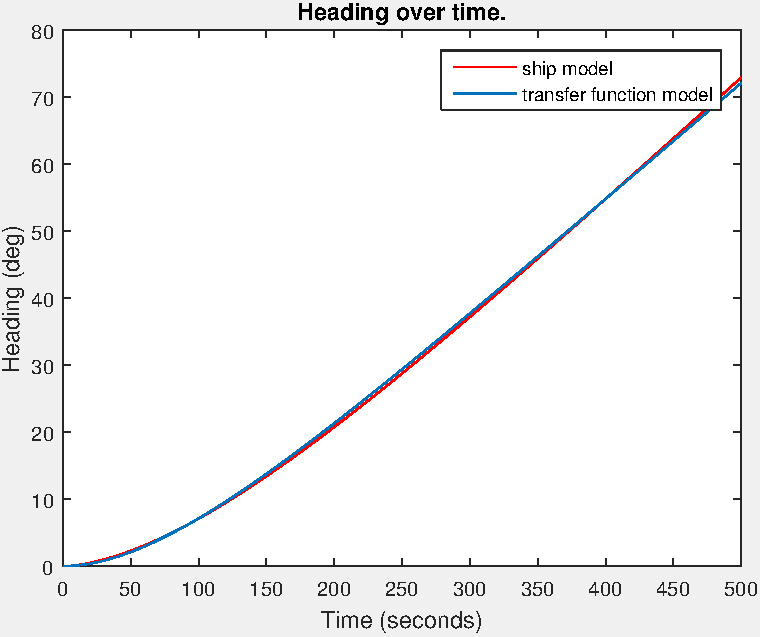
\includegraphics[width=0.5\textwidth]{images/1d-riktig_amplitude}
    \caption{Welch PSD estimate}
    \label{fig:1d-riktig_amplitude}
\end{figure}